% SPAR Report Template
% Compatible with arXiv (TeX Live 2023+, pdflatex)
%
% To compile: latexmk -pdf spar-report.tex
% Or use the build scripts: build spar-report.tex

% ============================================================================
% DOCUMENT CLASS
% ============================================================================
% Options: midterm | final | arxiv
% - midterm: Title prefix "Midterm Report:", SPAR branding
% - final: Title prefix "Final Report:", SPAR branding
% - arxiv: No prefix, removes all SPAR-specific decoration
\documentclass[midterm]{sparreport}

% ============================================================================
% METADATA
% ============================================================================
\title{Your Report Title Here}

\author{
  \textbf{Author Name}\\
  \texttt{author@example.com}
  % Optional: Add institution/affiliation (especially for arXiv mode):
  % \\
  % Your Institution
  % Add more authors (displayed horizontally) with \and:
  % \and
  % \textbf{Second Author}\\
  % \texttt{second@example.com}\\
  % Second Institution
}

\sparround{Fall 2025}

% ============================================================================
% DOCUMENT BEGINS
% ============================================================================
\begin{document}

\maketitle

% ============================================================================
% ABSTRACT (100-200 words)
% ============================================================================
\begin{abstract}
% TODO: Write 100-200 word abstract summarizing your research question,
% methodology, and key findings/preliminary results.
Your abstract goes here. Briefly describe the problem, your approach, and main findings.
\end{abstract}

% Keywords (optional but recommended, especially for arXiv submission)
\keywords{alignment research \and machine learning \and AI safety}

% ============================================================================
% INTRODUCTION AND STATEMENT OF THE PROBLEM (100-350 words)
% ============================================================================
\section{Introduction and Statement of the Problem}
% TODO: Introduce the research area and clearly state the specific problem
% you're addressing. Provide context and motivation. (100-350 words)

Introduce your research area and the specific problem you're investigating.

% ============================================================================
% METHODOLOGY (200-500 words)
% ============================================================================
\section{Methodology}
% TODO: Describe your research methods, experimental setup, datasets,
% algorithms, or analytical approaches. (200-500 words)

Describe your research approach and methods.

% Example figure reference
% \begin{figure}[htbp]
%   \centering
%   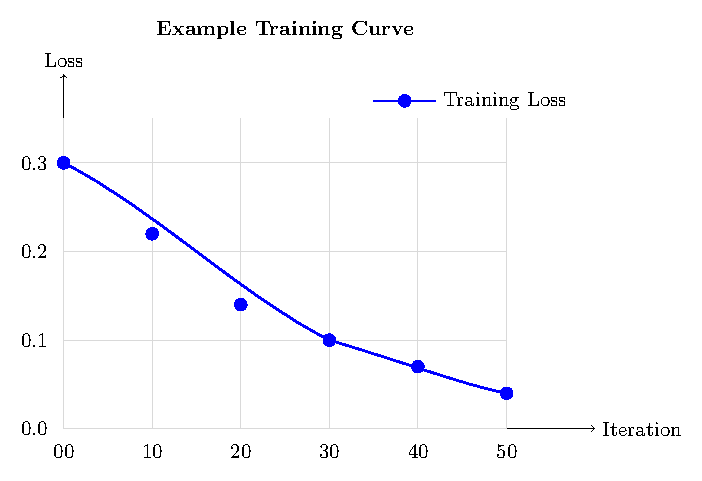
\includegraphics[width=0.7\textwidth]{figures/example-figure.pdf}
%   \caption{Example figure caption.}
%   \label{fig:example}
% \end{figure}

% Example table
% \begin{table}[htbp]
%   \centering
%   \caption{Example table caption.}
%   \label{tab:example}
%   \begin{tabular}{lcc}
%     \toprule
%     Method & Accuracy & Time \\
%     \midrule
%     Approach A & 85\% & 2.3s \\
%     Approach B & 92\% & 4.1s \\
%     \bottomrule
%   \end{tabular}
% \end{table}

% ============================================================================
% RESULTS (200-400 words)
% ============================================================================
\section{Results}
% TODO: Present your findings with figures, tables, and analysis.
% For midterm reports, preliminary/partial results are expected.
% For final/arxiv reports, present complete results. (200-400 words)

Present your results here.

% ============================================================================
% DISCUSSION (200-500 words)
% ============================================================================
\section{Discussion}
% TODO: Interpret your results, discuss implications, limitations,
% and connections to broader research questions. (200-500 words)

Discuss the implications and interpretation of your results.

% ============================================================================
% NEXT STEPS (150-400 words)
% ============================================================================
\section{Next Steps}
% TODO: Outline your plan for the remainder of the research program.
% What experiments, analyses, or extensions do you plan? (150-400 words)
% Note: For final reports or arXiv papers, you may delete this section or
% replace it with "Future Work" or "Conclusion".

Describe your planned next steps.

% ============================================================================
% BIBLIOGRAPHY
% ============================================================================
% For arXiv submission: You MUST include the generated .bbl file!
% Compile with: pdflatex -> bibtex -> pdflatex -> pdflatex
% Then submit both .tex and .bbl files to arXiv.

\bibliographystyle{plain}
\bibliography{references}

% Note: Authors can manually add sections like "Related Work", "Conclusion",
% "Acknowledgments", etc. when expanding this template for arXiv papers.

\end{document}
